\documentclass{beamer}
\usepackage{tikz, graphicx}
\usetikzlibrary{graphs, graphs.standard, positioning, quotes}

\mode<beamer>{
}

\theoremstyle{Plain}\newtheorem{kt}{Kuratowski's Theorem}
\theoremstyle{Definition}\newtheorem{te}{Tr\'emaux Exploration}
\theoremstyle{Definition}\newtheorem{dfs}{Depth-First Search}

\title{Introduction to Graph Theory}
\author{Brian Eft}
\date{June 29, 2021}
\institute{Tech Elevator Columbus}

\begin{document}
\begin{frame}
  \titlepage
\end{frame}

\begin{frame}
  \frametitle{Outline}
  \tableofcontents  
\end{frame}

% Introduction
\section{Introduction}
\begin{frame}
  \frametitle{Introduction}
    \begin{definition}
        \alert{Graph Theory} is a field of mathematics which studies mathematical structures called \emph{graphs}.
    \end{definition}
  
\end{frame}

% Basic Definitions
\subsection{Basic Definitions}
\begin{frame}
  \frametitle{What is a Graph?}
  \begin{definition}
    A \alert{graph} consists of two sets, $V$ and $E$. $V$ is a set of
    \emph{vertices}. $E$ is a set of unordered pairs of vertices, called
    \emph{edges}.
  \end{definition}

  \pause
  \begin{example}
  \begin{columns}
    \column{0.3\textwidth}
    \begin{center}
    \tikz {
      \node [draw, circle] (a) at (0,2) {a};
      \node [draw, circle] (b) at (0,0) {b};
      \node [draw, circle] (c) at (2,2) {c};
      \node [draw, circle] (d) at (2,0) {d};
      \graph {
        (a) -- (c);
        (a) -- (d);
        (b) -- (c);
        (b) -- (d);
      };
    }
    \end{center}
    \column{0.7\textwidth}
    Graph $G$ has a vertex set $V$ and edge set $E$.
    \begin{equation*}
      V = \{ a,b,c,d \}
    \end{equation*}
    \begin{equation*}
      E = \{\{a, c \}, \{a, d \}, \{b, c \}, \{b, d \}\}
    \end{equation*}
    \begin{equation*}
      E = \{ac,ad,bc,bd\}
    \end{equation*}
  \end{columns}
  \end{example}
\end{frame}

\begin{frame}
  \frametitle{Graph Representations}
  \begin{columns}
    \column{0.5\textwidth}
    \begin{center}
    \tikz {
      \node [draw, circle] (a) at (0,2) {a};
      \node [draw, circle] (b) at (0,0) {b};
      \node [draw, circle] (c) at (2,2) {c};
      \node [draw, circle] (d) at (2,0) {d};
      \graph {
        (a) -- (c);
        (a) -- (d);
        (b) -- (c);
        (b) -- (d);
      };
    }
    \end{center}
    \column{0.5\textwidth}
    \begin{center}
    \tikz {
      \node [draw, circle] (a) at (0,6) {a};
      \node [draw, circle] (b) at (0,2) {b};
      \node [draw, circle] (c) at (0,4) {c};
      \node [draw, circle] (d) at (0,0) {d};
      \graph {
        (a) -- (c);
        (a) --[bend right] (d);
        (b) -- (c);
        (b) -- (d);
      };
    }
    \end{center}
  \end{columns}
\end{frame}

\begin{frame}
  \frametitle{Simple, Multi, and Pseudographs}
  \begin{itemize}
    
  \item A \alert{simple graph} contains no duplicate edges or loops. A loop is when a vertex connects to itself.
  \pause
  \item If we allow multiple edges between a pair of vertices, we get a \alert{multigraph}.
    \begin{figure}[h]
    \tikz {
      \node [draw, circle] (a) at (0,0) {};
      \node [draw, circle] (b) at (2,0) {};
      \graph {
        (a) --[bend right] (b);
        (a) --[bend left] (b);
      };
    }
    \end{figure}

  \pause
  \item If we allow loops, we get a \alert{pseudograph}.
    \begin{figure}[h]
    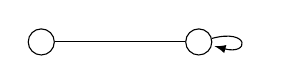
\begin{tikzpicture}
      \node [draw, circle] (a) at (0,0) {};
      \node [draw, circle] (b) at (2,0) {} edge [loop right, >=latex] node {} (x);
      \path (a) edge (b);
    \end{tikzpicture}
    \end{figure}
  \end{itemize}

\end{frame}

\begin{frame}
  \frametitle{Directed Graphs}
  If we make the edges of the graph a set of ordered pairs, we get a \alert{directed graph}, or digraph.
    \begin{figure}[h]
    \tikz {
      \node [draw, circle] (a) at (0,0) {a};
      \node [draw, circle] (b) at (1,2) {b};
      \node [draw, circle] (c) at (2,0) {c};
      \graph {
        (a) ->[bend right, >=latex] (b);
        (b) ->[bend right, >=latex] (a);
        (a) ->[>=latex] (c);
      };
    }
      \begin{equation*}
        E = \{\left( a,b\right) ,\ \left( b,a\right) ,\ \left( a,c\right) \}
      \end{equation*}
    \end{figure}
\end{frame}

% Motivation
\subsection{Motivation}
\begin{frame}
  \frametitle{Seven Bridges of K\"onigsberg}
  \begin{figure}[h]
  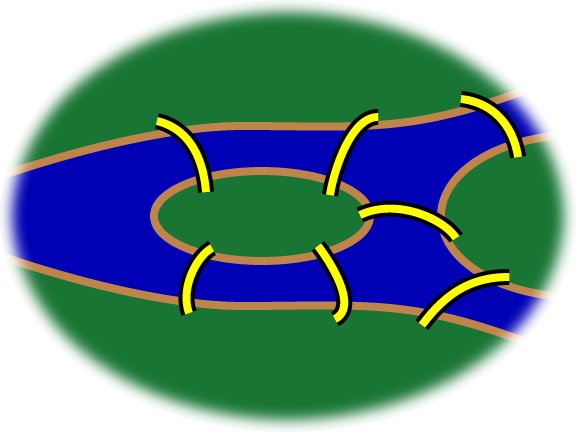
\includegraphics[height=.6\textheight]{images/7bridges.png}
  \end{figure}
  Find a walk through the city that crosses each bridge exactly once.
\end{frame}

\begin{frame}
  \frametitle{Three Utilities Problem}
  \begin{figure}[h]
  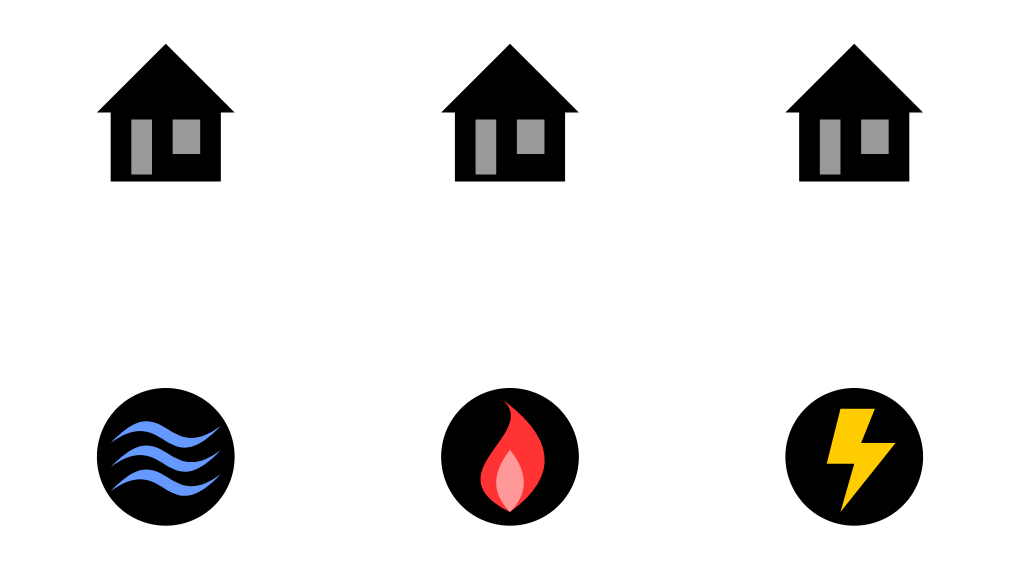
\includegraphics[height=.5\textheight]{images/3utilities.png}
  \end{figure}
  Connect every house to water, gas, and electric without crossing any lines.
\end{frame}

\begin{frame}
  \frametitle{Escaping a Maze}
  \begin{center}
  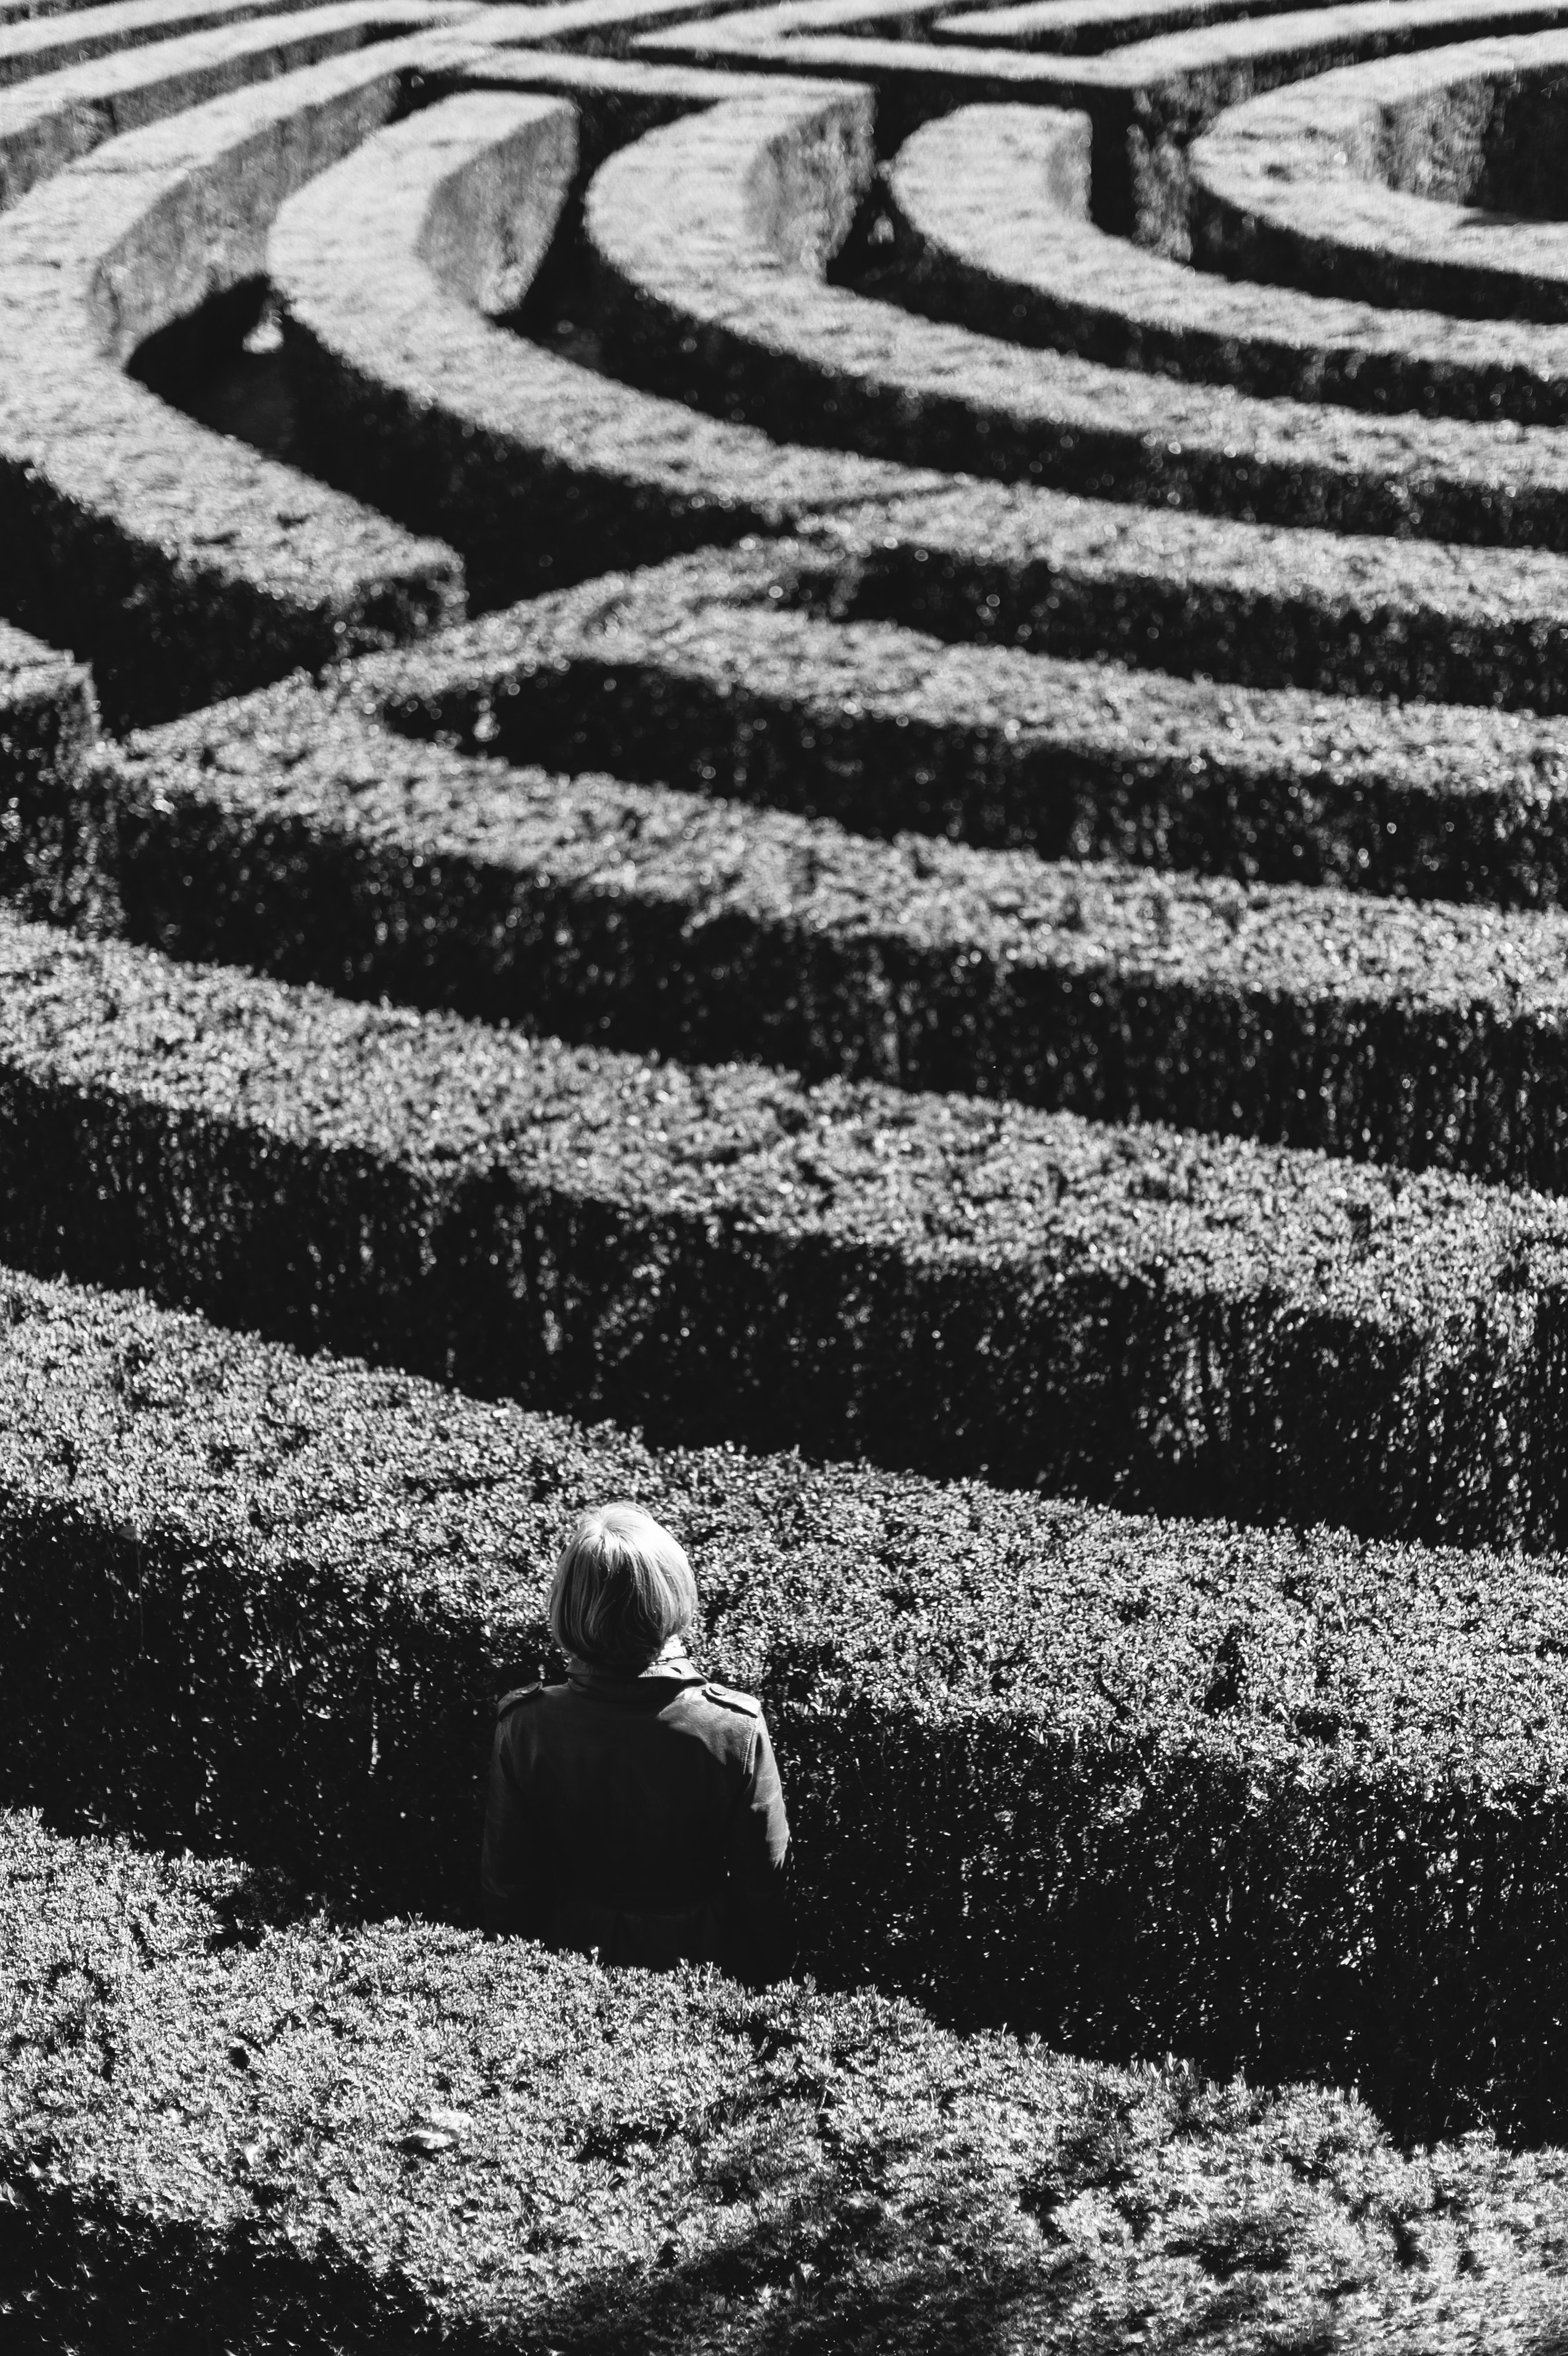
\includegraphics[width=0.4\textwidth]{images/hedge.jpg}
  \end{center}
\end{frame}



% Concepts
\section{Concepts}
% Euler Trails
\subsection{Euler Trails}
\begin{frame}
  \frametitle{Adjacency, Incidence, and Degree}
  \begin{itemize}
    \item Two vertices $u$ and $v$ are said to be \alert{adjacent} if there is an edge $uv$ connecting them. If there is no edge $uv$, then they are nonadjacent.
    \item If an edge has a vertex $v$ as an end vertex, we say that edge is \alert{incident} to $v$.
    \item The \alert{degree} of a vertex $v$ is the number of edges incident to $v$. 
  \end{itemize}
    \begin{figure}[h]
    \tikz {
      \node [draw, circle] (a) at (2,0) {a};
      \node [draw, circle] (b) at (3,2) {b};
      \node [draw, circle] (c) at (4,0) {c};
      \node [draw, circle] (d) at (1,2) {d};
      \graph {
        (a) -- (b);
        (a) -- (c);
        (a) -- (d);
        (b) -- (c);
      };
    }
    \begin{equation*}
      \deg{\left( a \right)} = 3
    \end{equation*}
    \end{figure}
\end{frame}

\begin{frame}
  \frametitle{Walks, Paths, and Trails}
  \begin{itemize}
    \item A \alert{walk} in a graph is a sequence of vertices such that each consecutive pair of vertices in the sequence are adjacent. The vertices need not be distinct.
    \item A walk with distinct vertices is called a \alert{path}.
    \item A walk with distinct edges is called a \alert{trail}.
  \end{itemize}
  \begin{figure}[h]
  \tikz {
      \node [draw, circle] (a) at (2,0) {a};
      \node [draw, circle, gray] (b) at (3,2) {b};
      \node [draw, circle] (c) at (4,0) {c};
      \node [draw, circle] (d) at (1,2) {d};
      \graph {
        (a) --[gray] (b);
        (a) -- (c);
        (a) -- (d);
        (b) --[gray] (c);
      };
    }
  \begin{equation*}
    d,\ a,\ c
  \end{equation*}
  \end{figure}
\end{frame}

\begin{frame}
  \frametitle{Seven Bridges of K\"onigsberg Revisited}
  \begin{columns}
    \column{0.35\textwidth}
    \begin{center}
    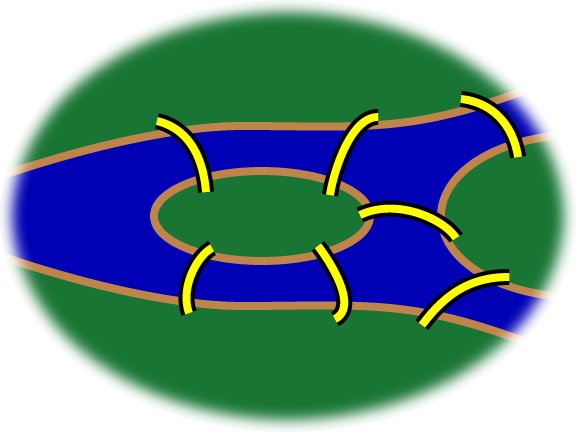
\includegraphics[width=\textwidth]{images/7bridges.png}
    \newline
    \newline
    \tikz {
      \node [draw, circle] (a) at (0,1) {};
      \node [draw, circle] (b) at (1,0) {};
      \node [draw, circle] (c) at (0,-1) {};
      \node [draw, circle] (d) at (-1,0) {};
      \graph {
        (a) -- (b);
        (b) -- (c);
        (c) --[bend left] (d);
        (c) --[bend right] (d);
        (d) --[bend left] (a);
        (d) --[bend right] (a);
        (b) -- (d);
      };
    }
    \end{center}
  \column{0.65\textwidth} 
  \pause
    \begin{itemize}
      \item Is there a trail which includes every edge?
      \item Known today as an Euler walk or Eulerian trail
      \item Leonhard Euler (1707--1783)
        \pause
      \item An undirected graph has an Euler walk if and only if exactly zero or two vertices have odd degree.
    \end{itemize}
  \end{columns}
\end{frame}


% Graph Planarity
\subsection{Graph Planarity}
\begin{frame}
  \frametitle{Complete Graphs}
  A graph is \alert{complete} if every vertex is adjacent to every other vertex.
  \begin{figure}[h]
    \tikz \graph [nodes={draw, circle}, empty nodes] { subgraph K_n [n=2] };
    \tikz \graph [nodes={draw, circle}, empty nodes] { subgraph K_n [n=3, clockwise] };
    \tikz \graph [nodes={draw, circle}, empty nodes] { subgraph K_n [n=4, clockwise] };
    \tikz \graph [nodes={draw, circle}, empty nodes] { subgraph K_n [n=5, clockwise] };
    \begin{equation*}
      K_2,\ K_3,\ K_4,\ \text{and }K_5
    \end{equation*}
  \end{figure}
\end{frame}

\begin{frame}
  \frametitle{Bipartite Graphs}
  A graph is \alert{bipartite} if all vertices can be colored red or blue such that every edge connects a red vertex to a blue vertex.
  \begin{figure}[h]
    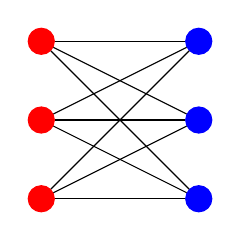
\begin{tikzpicture}[new set=red, new set=blue]
      \foreach \i in {1,2,3} {
        \node [draw, circle, fill, red, set=red] (r\i) at (0,\i) {};
        \node [draw, circle, fill, blue, set=blue] (b\i) at (2,\i) {};
      }
      \graph {
        (red) -- [complete bipartite] (blue)
      };
    \end{tikzpicture}
    \[K_{3,3}\]\\
    The complete bipartite graph of $3$ red vertices and $3$ blue vertices.
  \end{figure}
\end{frame}

\begin{frame}
  \frametitle{Graph Planarity}
  \begin{columns}
    \column{.4\textwidth}
    \begin{figure}
    \tikz \graph [nodes={draw,circle}, empty nodes] { subgraph C_n [n=3, clockwise] -- mid };
  \end{figure}
  \column{.6\textwidth}
    A graph is \alert{planar} if it can be drawn on a plane in such a way that edges do not intersect, except at vertices. 
  \end{columns}

  \begin{columns}
    \column{.4\textwidth}
    \tikz \graph [nodes={draw, circle}, empty nodes] { subgraph K_n [n=5, clockwise] };
    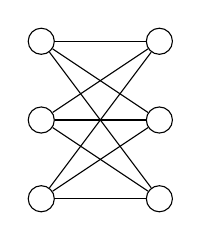
\begin{tikzpicture}[new set=red, new set=blue]
      \foreach \i in {1,2,3} {
        \node [draw, circle, set=red] (r\i) at (0,\i) {};
        \node [draw, circle, set=blue] (b\i) at (1.5,\i) {};
      }
      \graph {
        (red) -- [complete bipartite] (blue)
      };
    \end{tikzpicture}
    \column{.6\textwidth}
  \begin{kt}
    A graph $G$ is planar if and only if it contains no subdivision of $K_5$ or $K_{3,3}$.
  \end{kt}
  \end{columns}
\end{frame}


% Graph Algorithms
\subsection{Graph Algorithms}
\begin{frame}
  \frametitle{Labyrinth of Daedalus}
  \begin{columns}
    \column{0.5\textwidth}
    \includegraphics[width=\textwidth]{images/Theseus.jpg}
  
    \column{0.5\textwidth}
    \begin{itemize}
      \item Graph = maze\\ Vertex = intersection\\ Edge = passage
      \item How to search for the exit in a maze without getting lost and wandering in circles?
      \item Legend of Theseus and the Minotaur
    \end{itemize}
  \end{columns}
\end{frame}

\begin{frame}
  \frametitle{Graph Search}
    \begin{te}
    \begin{enumerate}
      \item Follow any unmarked passage, unspooling string behind you
      \item Mark all passages and intersections when first visiting them
      \item Backtrack by rewinding the string when you approach a marked intersection
      \item Backtrack when no unvisited options remain at an intersection
      \item Repeat until the exit is found, or the entire maze is explored
    \end{enumerate}
    \end{te}
    \pause

    \begin{dfs}
    \begin{enumerate}
      \item Mark vertex as visited
      \item Recursively visit all adjacent unmarked vertices
    \end{enumerate}
    \end{dfs}
\end{frame}

\begin{frame}
  \frametitle{Shortest Path}
  An \alert{edge-weighted graph} is a graph where each edge has a weight or cost.
  \begin{figure}
    \tikz {
      \node [draw, circle] (a) at (0,2) {a};
      \node [draw, circle] (b) at (0,0) {b};
      \node [draw, circle] (c) at (2,2) {c};
      \node [draw, circle] (d) at (2,0) {d};
      \node [draw, circle] (e) at (4,2) {e};
      \node [draw, circle] (f) at (4,0) {f};
      \node [draw, circle] (g) at (6,0) {g};
      \graph {
        (a) --["10"] (c);
        (a) --["15"] (b);
        (b) --["8"] (d);
        (c) --["18"] (e);
        (c) --["22"] (d);
        (d) --["12"] (f);
        (e) --["5"] (f);
        (e) --["28"] (g);
        (f) --["13"] (g);
      };
    }
  \end{figure}
  A \emph{shortest path algorithm} finds a path between two vertices with the minimum cost.
\end{frame}

\section{Conclusion}
\subsection{Real-World Problems}
\begin{frame}
  \frametitle{Real-World Problems}
  \begin{itemize}
    \item Maps
    \item Webpages
    \item Electric Circuits
    \item Social Networks
    \item Scheduling
    \item Commerce
      \begin{description}
        \item[Arbitrage]: shortest-path algorithm
      \end{description}
  \end{itemize}
\end{frame}

\section{References}
\begin{frame}
  \frametitle{References}
  \begin{thebibliography}{99}
    \bibitem{cgt} Harris, John M., Hirst, Jeffry L., and Michael J.
      Mossinghoff. 2008. \emph{Combinatorics and Graph Theory}. New
      York: Springer.
    \bibitem{a} Sedgewick, Robert, and Kevin Wayne. 2011.
      \emph{Algorithms}. Upper Saddle River: Pearson Education.
  \end{thebibliography}
\end{frame}

\end{document}
